\documentclass[10pt]{article}
\usepackage{xeCJK}
\setCJKmainfont{Noto Serif CJK SC}
\setCJKsansfont{Noto Sans CJK SC}
\setCJKmonofont{Noto Sans Mono CJK SC}
\usepackage[a4paper,margin=20mm]{geometry}
\usepackage{amsmath,amssymb,booktabs,graphicx,microtype,url}
\usepackage[section]{placeins}
\usepackage[hidelinks]{hyperref}
\usepackage[numbers,sort&compress]{natbib}
\renewcommand{\abstractname}{摘要}
\renewcommand{\figurename}{图}
\renewcommand{\tablename}{表}
\renewcommand{\refname}{参考文献}
\setlength{\emergencystretch}{2em}
\graphicspath{{../../results/figures/}}
\newcommand{\TaskCount}{60}
\newcommand{\CandidateCount}{300}
\newcommand{\KilledCount}{202}
\newcommand{\ControlCount}{98}
\newcommand{\IWCCBA}{88.12}
\newcommand{\EndpointBA}{77.48}
\newcommand{\GainPoints}{10.64}
\newcommand{\GainCILow}{8.88}
\newcommand{\GainCIHigh}{12.50}
\newcommand{\PermutationP}{1.0\times10^{-5}}
\newcommand{\IWCCRecall}{76.24}
\newcommand{\IWCCSpecificity}{100.00}
\newcommand{\ClauseCount}{71}
\newcommand{\TraceCount}{77}
\newcommand{\MedianRuntime}{0.487}
\newcommand{\RuntimeThroughput}{1715}


\title{从轨迹到见证契约：面向 LLM Agent 技能的增量式前置条件--效果编译}
\author{匿名作者}
\date{匿名稿，2026 年 9 月}

\begin{document}
\maketitle

\begin{abstract}
可复用 Agent 技能越来越多地以可执行动作程序保存，但这些程序通常没有可机器检查的前置条件与效果说明。因此，一个修改即使保留了看似正确的终点动作，也可能破坏导航、持有关系或变换依赖。本文提出增量式见证契约编译（Incremental Witnessed Contract Compilation, IWCC）：从成功执行轨迹中编译关于目标角色、必需里程碑、先后关系、导航以及生产者--消费者数据流的确定性契约，并为每条学习到的约束保留证据来源。IWCC 在调用环境前检查完整候选程序，返回违规约束及动作位置；它不负责规划或修复。方法开发仅使用已暴露的历史证据。随后，我们在选择新任务前冻结编译器、主要对照、模型版本、统计方法和通过门槛，并对 \TaskCount{} 个与既有实验零重叠的 ALFWorld 与 ScienceWorld 原生任务进行独立确认。四种结果盲变异产生 240 次原生重放；连同健康程序和自然存活变体，共有 \CandidateCount{} 个候选、\KilledCount{} 个被原生环境杀死的修改和 \ControlCount{} 个对照。IWCC 的平衡准确率为 \IWCCBA\%，最强对照为 \EndpointBA\%，绝对提高 \GainPoints{} 个百分点（任务分层 95\% 区间为 \GainCILow--\GainCIHigh{} 个百分点；配对置换 $p=\PermutationP$）。其召回率为 \IWCCRecall\%，\ControlCount{} 个对照全部通过，且两个环境中的方向均为正。单 CPU 进程的验证中位耗时为 \MedianRuntime{} ms。结果支持一个有边界的结论：带轨迹见证的结构契约可以低误报、可审计地预检可执行技能修改，但不能证明语义成功，也不能替代原生测试。
\end{abstract}

\noindent\textbf{关键词：} 大语言模型智能体；Agent 技能；规约挖掘；前置条件--效果契约；回归验证；执行轨迹

\section{引言}
大语言模型智能体正将有用行为保存为自然语言流程、脚本、动作程序及相关资源组成的可复用技能。程序化技能可以减少重复推理并改善迁移 \citep{wang2025asi,guo2026skilldisco}，显式激活、执行与终止条件则有助于提高复用可靠性 \citep{mi2026skillpro}。但持久化也改变了故障性质：一个错误程序不再只造成一次失败，而可能被反复调用、与其他技能组合，并进入后续版本。

许多技能工件只有任务目标和动作列表，缺少把二者连接起来的可执行契约。例如，一个家务技能需要拿取杯子、在冰箱中冷却并放入橱柜。修改后的程序可能仍含有最终放置动作，却漏掉拿取步骤、走到错误设备，或在已经失去对象后继续变换。文本依然流畅，终点检查也可能找到全部目标词。原生重放能够发现问题，但它可能昂贵、具有状态或带来真实副作用。因此，技能库需要一种在调用工具前解释结构冲突的低成本预检。

已有研究提供了关键基础。NSI 将轨迹提升为具有控制流和变量绑定的神经符号程序 \citep{shao2026nsi}；SKILL-DISCO 把成功路径蒸馏为可复用有限状态子图 \citep{guo2026skilldisco}；SkillOps 使用类型化契约维护技能库 \citep{pu2026skillops}；GraSP 以带前置条件和效果的图支持组合与局部修复 \citep{xia2026grasp}。Contractual Skills 将治理义务写入技能文档 \citep{liu2026contractual}，契约漂移研究则检查外部环境中的角色化假设 \citep{fan2026drift}。然而，一个更窄但实际的问题仍缺少独立验证：能否从成功原生轨迹增量编译紧凑契约，为每条约束保留证据，并在不执行候选程序的条件下区分真实失效修改与健康或行为等价修改？

本文提出 IWCC。环境适配器把原生命令解析为类型化事件；公开目标绑定对象、目的地、变换设备和测量对象等语义角色；成功轨迹见证必需里程碑及先后关系；轻量抽象解释器检查持有、位置、导航和终端角色效果。每条学习到的约束都带有成功轨迹哈希，集合式合并保证规范契约不受轨迹输入顺序影响。

本文贡献如下：
\begin{itemize}
  \item 提出统一目标角色、里程碑、顺序、导航和数据流的轨迹到契约编译器；
  \item 引入逐约束证据溯源和顺序无关的确定性要求，使动态挖掘结果可以审计；
  \item 在冻结主要对照、模型版本和统计方法后，完成跨两个原生环境的零重叠独立确认；
  \item 证明该契约能在亚毫秒级 CPU 延迟下提高缺陷筛查能力，同时保留健康与行为等价程序。
\end{itemize}

研究问题为：\textbf{RQ1} IWCC 能否比终点规则、顺序规则、轨迹相似度和本地语言模型更准确地识别原生失效修改？\textbf{RQ2} 它能否保留有效程序，并在不同环境和变异算子上保持正向效果？\textbf{RQ3} 其决策是否具备预执行场景所需的可审计性和低成本？

\section{相关工作}
\paragraph{程序化技能归纳。}
ASI 在线归纳和验证网页程序技能 \citep{wang2025asi}。NSI 从轨迹合成具有显式控制流和变量绑定的逻辑程序 \citep{shao2026nsi}；SKILL-DISCO 把共享成功结构表示为参数化有限状态子图 \citep{guo2026skilldisco}。Skill-Pro 定义技能的激活、执行和终止条件，并通过学习门禁验证候选 \citep{mi2026skillpro}。SCALAR 利用强化学习反馈迭代修正符号前置条件与效果 \citep{zabounidis2026scalar}。这些方法主要学习或执行技能；IWCC 固定候选动作程序，评估契约本身能否在发布前检出缺陷。

\paragraph{技能契约与生命周期维护。}
SkillOps 用前提、结果、动作、验证和失败组成类型化契约 \citep{pu2026skillops}；Contractual Skills 为人类可读技能包增加权限、证据、审批和输出义务 \citep{liu2026contractual}；契约漂移检测关注角色化外部假设 \citep{fan2026drift}。GraSP 用前置条件--效果有向无环图进行编排和局部修复 \citep{xia2026grasp}，SkillFuzz 提取契约以搜索跨技能隐式意图 \citep{hu2026skillfuzz}。IWCC 与其互补：研究单个技能内部的动作程序修改，以成功轨迹哈希支撑约束，并用原生行为结果检验执行前判定。

\paragraph{动态规约挖掘。}
从运行轨迹中挖掘时间规约和可能不变量是软件工程中的成熟思想 \citep{ammons2002mining,ernst2007daikon,beschastnikh2011synoptic}。动态证据不能证明普遍正确，所得性质只对观察到的执行和声明范围成立。IWCC 延续这一边界：契约是特定技能族的见证不变量，而不是对所有未来环境的定理。为检验成功轨迹过拟合，我们把健康程序和原生存活修改作为负例。

\section{问题定义}
令任务 $x=(e,f,o,s_0)$，其中 $e$ 为环境，$f$ 为技能族，$o$ 为公开目标，$s_0$ 为公开初始观察。完整候选程序为 $P=(a_1,\ldots,a_T)$。原生执行给出成功变量 $Y(P,x)\in\{0,1\}$，但预执行验证器不能访问 $Y$。

成功轨迹 $\tau=(x,P,\mathcal{O})$ 包含动作与观察。编译器从 $D^+=\{\tau_i:Y(P_i,x_i)=1\}$ 生成族契约 $C_{e,f}$。验证器输出 $V(C,x,P)=(d,L)$，其中 $d$ 为有效或损坏，$L$ 为带程序位置的违规列表。若健康源程序成功而修改程序失败，则称该修改被原生环境“杀死”；健康程序与修改后仍成功的程序均为对照。

主要终点为平衡准确率
\[
\mathrm{BA}=\tfrac12\left(\frac{TP}{TP+FN}+\frac{TN}{TN+FP}\right).
\]
该指标适合自然存活导致的类别不均衡。验证器不能通过普遍拒绝换取召回，因此另设召回率和误拒率门槛。

\section{增量式见证契约编译}
\subsection{类型化事件与目标角色}
环境适配器将命令规范化为事件 $q=(\mathrm{op},u,v)$，支持导航、开关、拿取、放置、清洗、冷却、加热、聚焦、测量和使用。具体实例（如 \texttt{drawer 4}）在状态流中保持不同；只有匹配任务角色时才移除数字后缀。这避免了开发版中不同物理容器被错误合并的问题。

目标解析器生成 $g=(f,r_s,r_d,r_t,k)$，包含技能族、对象角色、目的地角色、可选变换和数量。对 ScienceWorld 开放类别任务，首次符合条件的聚焦动作绑定具体对象，并向拿取和放置传播；温度计任务还绑定工具角色与条件分支目的箱。

\subsection{里程碑与轨迹见证}
每条成功轨迹被抽象为里程碑序列 $M(\tau)$，例如拿取对象、冷却对象和放置对象。支持度不低于 $\theta_m=0.8$ 的里程碑成为必需条件；支持度不低于 $\theta_o=0.9$ 且不存在反向观察的关系形成先后约束。成功的替代序列被保留为分支，不会因为偏离多数路径而直接判错。

每条必需或顺序约束 $c$ 保存见证集合
\[
W(c)=\{h(\tau):\tau\text{ 支持 }c\},
\]
其中 $h$ 是轨迹身份、目标、初始观察与动作序列的 SHA-256。ScienceWorld 导航边也保留见证。最终契约由 \TraceCount{} 条成功开发轨迹支撑，包含 \ClauseCount{} 条必需、顺序和导航约束。轨迹按哈希去重，支持度由集合统计，因此任意输入排列都得到同一个规范哈希；开发阶段 100 次随机排列完全一致。

\subsection{预执行抽象解释}
验证器先检查目标绑定的必需里程碑，再检查先后关系。IWCC 进一步单遍维护当前位置和所持具体实体。ALFWorld 的拿取动作要求当前位于来源容器；变换要求持有对象且位于正确设备；放置要求持有对象且当前位置等于目的地。ScienceWorld 的移动必须沿开发成功轨迹见证的导航边进行。每个违规项含约束、动作和下标。

验证仅使用 $C,e,f,o,s_0,P$，看不到任务编号、变异算子、健康参考程序或原生结果。其复杂度为 $O(|P|+|C_{e,f}|)$。通过只表示“没有发现已建模的结构违规”，而不是“任务必然成功”。

\section{实验设计}
\subsection{开发与冻结}
开发仅使用既有论文已暴露的 45 条健康轨迹和 135 条历史变异结果。32 条原生存活变体作为正向见证，防止契约拒绝有效替代路径。最终开发集有 103 个失效修改和 77 个对照，IWCC 的 BA 为 87.21\%，终点契约为 74.59\%。第一版编译器仅提升 7.77 个百分点，其失败来自实例名合并以及缺少 ScienceWorld 见证拓扑，相关结果完整保留。

在确认实验前，我们冻结源代码、阈值、契约、主要对照、提示词、模型版本、最近轨迹阈值、统计程序和十项门槛。第一次操作锁要求每个 ALFWorld 族 6 个任务，但某族排除历史样本后只剩 5 个，因而未生成名单或结果。第二个锁只调整族配额，仍保持每个环境 30 个任务和全部分析门槛；两个锁均保留供审计。

\subsection{独立原生确认}
冻结名单含 \TaskCount{} 个与历史证据零编号重叠的任务：ALFWorld 五个可靠任务族共 30 个，ScienceWorld 三个任务族的官方测试变体共 30 个 \citep{shridhar2021alfworld,wang2022scienceworld}。选择只读取环境、任务族、官方划分、兼容标记、历史排除和带种子的哈希排序。60 条专家/金标准轨迹全部成功。

在不知道结果时，为每个任务生成四种修改：删除末尾六步内按种子选中的可执行动作；与下一动作交换；截断最后三步；替换最后一个承载目标的目的地或设备角色。每次重放都重新初始化并核对完整初态签名。240 次原生重放均无技术错误，其中 202 个失败、38 个存活。加入 60 个健康程序后，最终有 \CandidateCount{} 个程序和 \ControlCount{} 个负例，没有按结果删样本。

\subsection{比较方法与统计}
终点契约检查目标所需里程碑，是预先指定的主要对照。顺序契约增加学习到的先后关系，但不执行状态流；最近成功轨迹以开发期固定阈值 0.6 判定规范化操作序列距离。Qwen3-4B-Instruct-2507、Phi-4-mini-instruct 和 Mistral-7B-Instruct-v0.3 三个固定版本模型接收同样的目标、初始观察和编号程序，以贪心解码输出有效、损坏或不确定；沿用开发规则，只有“损坏”算拒绝。

候选程序用于计分，但统计推断按共同源任务聚类。双侧配对符号置换使用 100,000 次固定种子抽样；分层 bootstrap 在环境--任务族内重采样任务，共 10,000 次。只有样本规模、BA、召回、误拒、至少 10 个百分点实际提升、区间、$p$ 值及双环境方向共十项门槛全部满足时才成稿。所有预测完成后，私有标签仅打开一次。

\section{结果}
\subsection{主要结果}
\begin{table}[t]
\centering
\caption{候选程序级的独立确认结果（\% ）。}
\label{tab:main-zh}
\begin{tabular}{lrrr}
\toprule
验证器 & 平衡准确率 & 召回率 & 特异度 \\
\midrule
终点契约 & 77.48 & 54.95 & 100.00 \\
顺序契约 & 77.48 & 54.95 & 100.00 \\
最近轨迹 & 50.74 & 1.49 & 100.00 \\
Qwen3-4B & 49.50 & 99.01 & 0.00 \\
Phi-4-mini & 50.72 & 86.14 & 15.31 \\
Mistral-7B & 51.12 & 60.40 & 41.84 \\
IWCC & 88.12 & 76.24 & 100.00 \\
\bottomrule
\end{tabular}
\end{table}


IWCC 的平衡准确率为 \IWCCBA\%，终点契约和顺序契约均为 \EndpointBA\%，绝对提高 \GainPoints{} 个百分点。任务分层 95\% 区间为 \GainCILow--\GainCIHigh{} 个百分点，任务配对置换 $p=\PermutationP$。IWCC 检出 202 个失效修改中的 154 个，召回率 \IWCCRecall\%；\ControlCount{} 个健康或原生存活程序全部通过。召回率 Wilson 95\% 区间为 69.91--81.58\%，零观测误拒对应的上端点为 3.77\%。十项冻结门槛全部通过。

三个模型裁判的 BA 为 49.50--51.12\%。Qwen 几乎拒绝所有程序，Phi 和 Mistral 也呈现较高误拒。这不代表模型的一般推理能力，而说明在低误报要求下，未经校准的生成式判断不能替代范围明确的结构契约。

\begin{figure}[t]
\centering
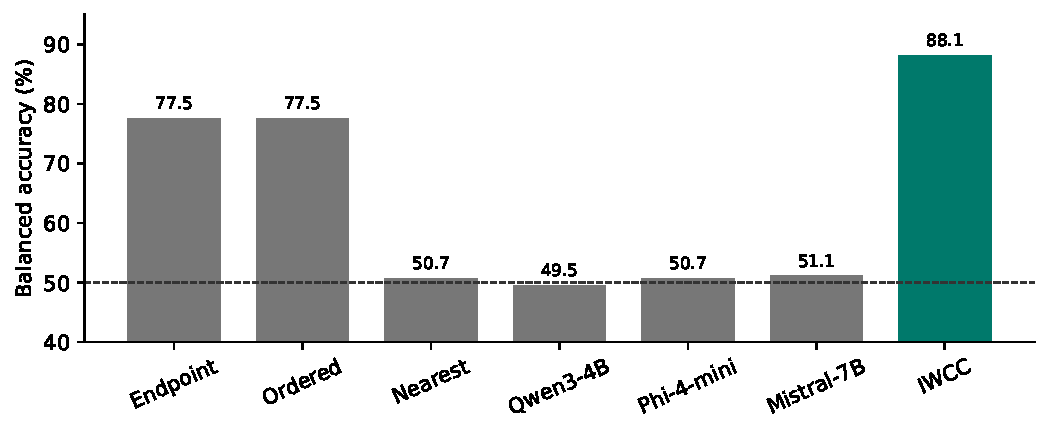
\includegraphics[width=0.98\linewidth]{balanced_accuracy.pdf}
\caption{独立原生确认上的平衡准确率。虚线表示随机水平，终点契约是最强对照。}
\label{fig:ba-zh}
\end{figure}

\subsection{环境、算子与定位}
\begin{table}[t]
\centering
\caption{分原生环境的平衡准确率（\% ）。}
\label{tab:environment-zh}
\begin{tabular}{lrrr}
\toprule
环境 & 终点契约 & IWCC & 增益 \\
\midrule
Alfworld & 79.39 & 95.61 & 16.23 \\
Scienceworld & 75.00 & 78.41 & 3.41 \\
\bottomrule
\end{tabular}
\end{table}


ALFWorld 中提升为 16.23 个百分点，ScienceWorld 为 3.41 个百分点。8 个任务族中 7 个为正、1 个持平，没有负向任务族。ScienceWorld 的 IWCC BA 仅为 78.41\%，因此总体结果不能被表述为所有细分场景均有强迁移。

对删除、相邻交换、截断和角色替换四种算子，IWCC 的失效召回分别为 72.55\%、74.19\%、80.00\% 和 76.67\%。终点契约对被杀死的相邻交换召回为 0，而 IWCC 为 74.19\%，直接体现了中间状态与数据流的价值。角色替换不是总体提升的唯一来源。

在 154 个已检出缺陷中，违规位置精确命中编辑动作的比例为 63.64\%，在前后 1 步内命中的比例为 94.16\%。单 CPU 进程 30,000 次调用的中位延迟为 \MedianRuntime{} ms，吞吐约 \RuntimeThroughput{} 程序/秒。三个模型对照共需 900 次 GPU 推理，峰值显存为 7.45--13.91 GiB；GPU 只用于比较实验，不是部署 IWCC 的必要条件。

\section{讨论}
\paragraph{实际使用方式。}
IWCC 适合放在技能修改和原生回归测试之间。若程序被拒绝，开发者可获得违规约束和位置；若通过，仍进入原生测试或风险受限发布门禁。这样可以在调用外部工具前过滤明显结构缺陷，同时不把静态契约伪装成语义执行器。轨迹哈希使维护者能够追查约束来源，并在证据过期时删除或更新。

\paragraph{终点规则为何不足。}
终点规则只能发现正确目标动作是否出现，无法判断智能体是否到达相应位置、是否仍持有对象，或导航路径是否受成功经验支持。相邻交换保留动作词汇和多数里程碑，因此终点与单纯顺序规则总体结果相同。抽象状态把生产动作和消费动作连接起来，无需记忆完整轨迹即可发现这类缺陷。

\paragraph{生命周期边界。}
契约编译回答技能在结构上承诺什么，但不回答需要多少原生证据才能发布，不自动修复被拒程序，也不分析多个技能之间的冲突。这些属于二维研究矩阵中的其他独立问题。明确边界能够避免把规划、验证、修复和治理都归功于同一个工件。

\section{有效性威胁}
\paragraph{构念有效性。}
受控变异不等同于真实技能缺陷。角色替换可能比语义逻辑错误更容易，而部分删除搜索动作在原生环境中仍然成功。本文以原生重放确定实际标签，并保留全部存活变体，但仍需在真实仓库版本上评估。

\paragraph{内部有效性。}
开发证据已暴露，只用于选方法。确认任务与历史编号零重叠；代码、对照、提示词、统计与门槛均在结果前哈希冻结。V2 名单锁的配额原因已公开。信息边界审计确认所有验证器不读取私有标签。确定性专家路径降低了随机噪声，但不代表随机 LLM 策略。

\paragraph{外部有效性。}
实验覆盖两个文本模拟器、8 个确认任务族和可解析动作程序，不覆盖网页 DOM 变化、代码智能体、任意 Shell 程序、并发技能、隐藏权限或随机 API。ScienceWorld 的较小收益和一个持平任务族说明，轨迹见证导航并不足以解决所有领域问题。

\paragraph{统计有效性。}
同一任务的多个候选彼此相关，因此显著性检验使用任务级配对效应，bootstrap 也按任务分层。60 个任务对任务族级精度仍有限。100,000 次置换使可报告 $p$ 值下限约为 $10^{-5}$。主结论以冻结的增益 bootstrap 为准，Wilson 区间仅作描述。

\section{复现说明}
工件包含源码、单元测试、两个方法锁、零重叠名单、60 条健康轨迹、240 个变异规格与全部结果、公开/私有候选分离、900 个模型输出、版本和哈希、分析结果及双语稿件。ALFWorld 游戏文件和模型权重仅以路径及版本引用，不重新分发。原生重放需要相邻的 Paper 01 模拟器资源；已发布记录的分析只需 CPU。实验环境为单张 RTX 3090、Python 3.12、PyTorch 2.8.0、CUDA 12.8、ALFWorld 0.4.2、ScienceWorld 1.2.3 和 OpenJDK 17。

\section{结论}
可执行 Agent 技能不能只有看似合理的动作列表。IWCC 将成功轨迹编译为确定、可溯源的结构契约，并在执行前检查修改。在冻结、零重叠的 ALFWorld/ScienceWorld 独立确认中，它比最强对照提高 \GainPoints{} 个百分点，任务聚类区间为正，且 \ControlCount{} 个对照中没有观测到误拒。本文结论保持克制：见证契约能够低成本、可审计地暴露已建模结构缺陷；未建模语义和真实可靠性仍必须由原生执行验证。

\bibliographystyle{plainnat}
\bibliography{../references}

\appendix
\section{冻结门槛与信息边界}
机器可读结果逐项记录十个确认条件。名单选定后没有替换任务，模型的“不确定”和错误拒绝均完整保留。公开候选文件只有候选编号、环境、任务族、目标、初始观察和程序；任务定位、变异算子、编辑下标、原生得分和失效标签仅位于后验分析器打开的私有文件。

\end{document}
